\newpage
\sect{Videoplattformen und ihre Veröffentlichungsvarianten}

\sub{Bereitstellungsvarianten}
Grundsätzlich gibt es 4 verschiedene Möglichkeiten der Filmbereitstellung: \\

\begin{itemize}
  \item Selbst gehostete Filme auf eigener Webseite.
  \item Fertig produzierter Film auf Videoplattform
  \item Livestream auf Videoplattform
  \item Youtube Premiere
\end{itemize}
{\vspace{-0.7cm}}

\subsub{Selbst gehostete Filme auf eigener Webseite}
Hierbei werden die eingereichten Filme auf der eigenen Webpräzens gezeigt.\\
Die Filmdateien können hierbei auf dem eigenen Server liegen oder über einen CDN zur Verfügung gestellt werden. \\
Content Delivery Networks haben hierbei den Vorteil das die Netzwerkauslastung des eigenen Webseiten-Servers gering bleibt. \\

Bekannte CDN's sind Akamai, Microsoft Azure, Amazon Web Services (AWS) sowie Cloudflare.

\subsub{Fertig produzierter Film auf Videoplattform}

Beim fertig produzierten Video auf einer Videoplattform ist es ähnlich wie beim hosten auf einem CDN. Der eigene Server wird entlastet aber zusätzlich stehen dem Nutzer häufig unteschiedliche Videoauflösungen zur Verfügung. Das ist ein großer Vorteil für Zuschauer welche über ein Mobiltelefon zuschauen möchten. Dort sind sie höheren Auflösungen oft nicht nötig und falls der Zuschauer über seinen Mobilfunkvertrag schaut wird sein Datenvolumen geschont. \\
Ein Nachteil können aber die AGB's des Anbieters sein und es kann vorkommen das Videos fälschlicherweise gesperrt werden.

\subsub{Livestream auf Videoplattform}
Im Unterschied zum fertig produzierten Video kann das Video zumindest während des erstmaligen Vorführen nicht geblockt werden.
Danach gibt es für den Verbleib des Videos verschiedene Möglichkeiten. \\
Bei manchen Plattformen ist das Video nur während des Livestreams zu sehen, bei anderen Plattformen ist das gestreamte Video auch danach noch ansehbar.\\

Beim Livestream müssen die Daten in Echtzeit zum Server übertragen werden.
Die maximale Bildqualität hängt daher stark von dem zur Verfügung stehenden Internetanschluss ab.
Während des Livestreams ist es möglich einen Livechat zur nutzen.
Auch wenn die Datenrate durch den Upload begrenzt ist hat man die Möglichkeiten einen Film in eine Anmoderierung sowie nachfolgende Diskussionsrunde einzubinden.




\subsub{Youtube Premiere}
Eine Youtube Premiere ist ein Mix aus vorproduziertes Video und Livestream.
Das vorproduzierte Video kann zum Zeitpunkt der Veröffentlichung nicht vorgespult werden.
Es ist möglich einen Livechat zu aktivieren um während der Vorführung zu kommunizieren.




\newpage
\sub{Aktuelle Videoportale (Land, Erscheinungsjahr)}

Viele bekannte Portale wie Clipfish (DE), MyVideo (DE), Sevenload(DE), Vevo (USA) gibt es nicht mehr.\\
Vevo vertreibt seine Videos nun über Youtube.\\


\begin{itemize}
  \item Europa
  \begin{itemize}
    \item alugha(DE 2014) kostenpflichtig und es sind nur 180 Minuten frei.
    \item item Dailymotion (FR 2005) Kein Livestreaming und die Videoübersicht ist recht unübersichtlich gestaltet.
  \end{itemize}
  \item Noch in Europa
  \begin{itemize}
    \item LiveLeak (GB 2006) verlinkt nur noch auf Youtubevideos
  \end{itemize}
  \item Amerika
  \begin{itemize}
    \item Twitch (USA 2011 Amazon) Streaming für Spieler,
    \item Vimeo (USA 2004) kostenpflichtig Livestreams erst ab 70€ im Monat,
    \item Youtube (USA 2005 Alphabet)
  \end{itemize}
  \item Asien
  \begin{itemize}
    \item Youku (China 2006) Nur in chinesischer Sprache
    \item TikTok (China 2016) Nur Miniclips
  \end{itemize}
\end{itemize}


{\vspace{0,2cm}}
\textbf{Fazit:}
Bleibt prinzipiell nur Youtube ...

\sub{Fazit: Youtube}

Youtube ist eine Videoplattform welche von Youtube LLC betrieben wird. \\
Youtube LLC eine Tochtergesellschaft von Google LLC, die wiederum eine Tochtergesellschaft von Alphabet Inc. ist.

\begin{flushright}
  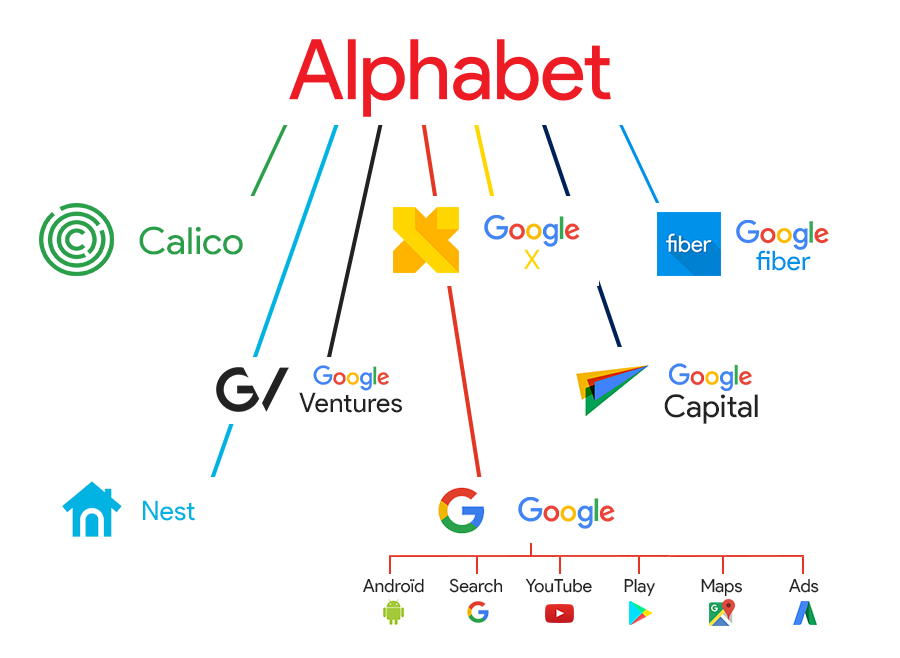
\includegraphics[scale=1.3]{./pictures/alphabet.png}
\end{flushright}

{\vspace{-2,5cm}}
Funktionen die Youtube bietet:
\begin{itemize}
  \item live-Streaming (mit Live-Chat)
  \item Produzierte Videos
  \item Video Premieren \\ (Vorproduzierte Videos. verhalten sich wie Livestream (mit Live-Chat, können nicht vorgespult werden bei der Premiere.))
\end{itemize}
\newpage

Neben der werbefreien Veröffentlichung können Videos auch Monetarisiert werden. Dies geschieht bei Youtube über den Google Dienst AdSense, welcher oft auch auf normalen Webseiten benutzt wird. \\
Hauptberufliche Youtuber nutzen diesen Dienst zwar auch, aber zum  \quote{Davon Leben} reicht dies in der Regel nicht.\\
Oftmals reichen die Einahmen hiervon gerade so um die Produktionskosten des Videos wieder rein zu holen. \\
Die meisten Youtuber finanzieren diese sich über Affiliate-Marketing-Links was einer Vermittlungsprovision entspricht. Hierbei werden Produktreviews gemacht und dann Links zu verschiedenen Shops in die Videobeschreibung gepackt über die der Youtuber dann ein paar Euro bekommt wenn der Zuschauer über diesen das Produkt kauft. \\
Ebenso ist es mittlerweile üblich das Firmen direkt Youtuber sponsern und im Gegenzug dann eine 1-3 minütige Produktvorstellung ins Video eingebunden bekommen.\\
Der Vorteil hierbei ist für beide Seiten das Google als \quote{Zwischenhändler} (Welche ja auch eine Provision möchte) wegfällt. \\
Dadurch bekommt der Youtuber in der Regel höhere Einnahmen als über Youtube. Die Firma kann hierdurch gezielter werben und ist nicht auf den Google-Algorithmus angewiesen.\\

Aber es gibt auch Youtube Netzwerke wie \quote{Funk} des öffentlich rechtlichen Rundfunks welche Youtuber sponsern.\\

Nennenswerte Beispiele sind hierbei:
\begin{itemize}
  \item maiLab von Mai Thi Nguyen-Kim produziert vom SWR
  \item Browser Ballett von Christian Brandes (und vielen weiteren) produziert von Steinberger Silberstein GmbH
  \item MrWissen2go von Mirko Drotschmann produziert von MDR und SWR
  \item STRG F ist ein wöchentliches Doku-Format welches vom NDR produziert wird
\end{itemize}


Funk finanziert aber auch viele Serien. Mit \quote{Wach} im Jahre 2018 wurde erstmalig ein Film finanziert

\newpage
\sub{Verschiedene Youtube-Streaming-Setups}
\begin{table}[h]
  \begin{adjustwidth}{-1cm}{-1cm}% adjust the L and R margins by 1 inch
    \begin{center}
      \textbf{Verschiedene Youtube Streaming Setups}
      \begin{tabular}{|p{3cm}|p{3cm}|p{3cm}|p{3cm}|p{3cm}|p{3cm}|}
        \hline
                          &  Geeignet für                                                         & Programmgestaltungsformat & Komplexität der Einrichtung & Erforderliche Mindestausrüstung & Anwendungsfall \\ \hline
        Mobilgerät        & Streaming unterwegs                                                   & Schnell und einfach       & Gering                      & Mobiltelefon mit Kamera & Livestream in wenigen Schritten über ein Handy startet \\ \hline
        Webcam            & Einfache Webcam-Streams                                               & Schnell und einfach       & Gering                      & Computer mit Webcam & Livestream mit wenigen Klicks starten\\ \hline
        Jetzt Streamen    & Reproduzierbare Livestreams, die eine einmalige Einrichtung erfordern & Produziert                & Mittel/Hoch                 & Computer mit Webcam und Streamingsoftware & Eine Liveadresse für wiederholbare Livestreams \\ \hline
        Veranstaltungen   & Livestream-Einrichtung mit vielen Anpassungsmöglichkeiten             & Tent-Poling-Video         & Hoch                        & Computer, Kamera, Streamingsoftware  & Eine benutzerdefinierte Live-Veranstaltung erstellen, welche auch ein Multicamstream sein kann. \\ \hline
        Youtube Premiere  & Produziertes Video mit Livechat                                       & Tent-Poling-Video         & Mittel/Hoch                 & Computer, Streamingsoftware & Ein einmalig nicht vorspulbares vorproduziertes Video welches Interaktionsmöglichkeiten bietet \\ \hline
      \end{tabular}
    \end{center}
  \end{adjustwidth}
\end{table}

















% \begin{table}[ht]
%   \begin{tabular}{|p{3cm}|p{3cm}|p{3cm}|p{3cm}|p{3cm}|}
%     \hline
%     &  Mobilgerät         & Webcam & Jetzt Streamen & Veranstalltungen \\ \hline
%     Geeignet für                    & Streaming unterwegs & Einfache Webcam-Streams & Reproduzierbare Livestreams, die eine einmalige Einrichtung erfordern & Livestream-Einrichtung mit vielen Anpassungsmöglichkeiten \\ \hline
%     Programmgestaltungsformat       & Schnell und einfach & Schnell und einfach & Produziert & Tent-Poling-Video \\ \hline
%     Komplexität der Einrichtung     & Gering & Gering & Mittel/Hoch & Hoch \\ \hline
%     Erforderliche Mindestausrüstung & Mobiltelefon mit Kamera & Computer mit Webcam & Computer mit Webcam und Streamingsoftware & Computer Kamera Streamingsoftware \\ \hline
%     Anwendungsfall                  & Livestream in wenigen Schritten über ein Handy starteb & Livestream mit wenigen Klicks starten & Eine Liveadresse für wiederholbare Livestreams & Eine benutzerdefinierte Live-veranstaltung erstellen, welche auch ein Multicamstream sein kann. \\ \hline
%   \end{tabular}
% \end{table}

% \begin{center}
% {\vspace{-15cm}}
